% we should list the event log definition and petri net definition
% also the process tree definition
% For definitions, we capitalize only the first character, others we use camel methods. 
This chapter introduces the most important concepts and notations that are used in this thesis. Firstly, the event data and process models typically used in process mining are described. Later, details of Inductive Miner techniques which relate to our work are listed.
\section{Event Log}
% introduce of event and trace , later event log historical business process execution data in information systems
Business processes in organizations can be reflected by their activities execution. The historical execution data is usually stored as event logs in information systems and can be used by process mining techniques to analyze, understand, and improve the business execution. To specify the event log, we begin with formalizing the various notations\cite{van2016data} .
\begin{definition}[Event]
	An event corresponds to one execution of an activity in business execution and written as $e$. An event is characterized by attributes, like a timestamp, activity name, associated costs, etc. The set of all possible events in a process is written as $\mathcal{E}$.
\end{definition}
\begin{definition}[Trace]
A trace is a finite sequence of events $\sigma \in \mathcal{E}^*$ with conditions that (i)  each event  appears only once in a trace. 
\[ \forall  1 \leq i,j \leq \vert \sigma \vert,  i \neq j \Rightarrow \sigma (i) \neq \sigma (j) \] 
(ii) one event can only appear in one trace. 
\[ \forall e \in \sigma, e \in \sigma\prime \Rightarrow \sigma = \sigma\prime \]  
\end{definition}
A trace also has a set of attributes, like its unique identifier, the cost. We extend this definition to handle traces with performance output according to certain KPIs. 
\begin{definition}[Labeled Trace]
A trace is labeled with respect to certain KPIs, if it has an attribute for the performance output. We call a trace positive, if the value of its performance attribute is positive, else the trace is negative.
\end{definition}
\begin{definition}[Event log and labeled Event log]
An event log $L$ is a set of traces, $L \in \mathcal{B(\mathcal{E}^*)}$. A labeled event log is an event log if all of its traces have an performance attribute according to certain KPIs.
\end{definition}
\section{Process Models}
After gathering an event log from the information system, process mining can discover a process model based on the event log, aims to improve the understanding of the business process. To describe the process, multiple process modeling languages are proposed in the last years, e.g, Petri net, BPMN models, etc. 

Among those model languages, Petri net has been best studied thoroughly. It captures concurrent systems in a compact manner. Process trees are based on a tree structure to organize the event relation and simple to understand in comparison with other models, like BPMN models. In this thesis, we use Petri net and process tree to represent our process.
\subsection{Petri Nets}
Petri nets are bipartite graphs which are built by \textbf{\emph{transitions}} represented by a square and \textbf{\emph{place}} in a circle. \textbf{\emph{Tokens}} in black dots are put in places to express the states of a Petri net. In the following, we define Petri nets in a formal way.
\begin{definition}[Petri net]
	A Petri net is a tuple $N=(P,T,F)$ where \\ P and T are disjoint finite set of  places and transitions, respectively, $P \cap T = \emptyset $. \\ F is the set of arcs to connect places and transitions, $F \subseteq (P\times T)\cup (T \times P)$.
\end{definition}
Further, we can define a labeling function $\lambda$ on the transitions.
\begin{definition}[Labeling function $\lambda$]	
	$\lambda$ is a function defined as 
	\[\lambda: T \rightarrow \Sigma \cup \{ \tau \}, \Sigma \text{ is a set of labels}, \tau \text{is an empty label}. \] 
\end{definition}
To express the dynamic states of Petri nets, we introduce a concept called \textbf{\emph{marking}}. 
\begin{definition}[Marking]
	A marking is a place multiset,$M:P \rightarrow N$, which assigns to a place a number of tokens. 
\end{definition}	
With marking concepts, we extend the form  $N=(P,T,F)$ and define a marked Petri net. 
\begin{definition}[Marked Petri nets]
A marked Petri net is a 4-tuple $N=(P,T,F,M_0)$ where $M_0$ is an initial marking of this net.
\end{definition}
If all the input places for a transition hold a token, the transition becomes enabled. In other words, the  activity in the corresponding process can be triggered. After this execution, the token in the input places are consumed and new tokens are generated in the output places. The firing sequence of transitions can carry out business execution in reality.  However, to perform the business on an enterprise level, the correctness of business process models is necessary. Soundness defines a minimum correctness criterion that a process model should satisfy\cite{van2006structural}. In the following, we give the definition of soundness for Petri nets.
\begin{definition}[Soundness]
	A Petri net is sound if and only if it satisfies the following conditions.
	\begin{itemize}
		\itemsep0em 
		\item safeness. Places cannot hold multiple tokens at the same time.
		\item proper completion. If the sink place is marked, all other places are empty.
		\item option to complete. It is always possible to reach the final marking just for the sink place.
		\item no dead part. For any transition there is a path from source to sink place through it. 
	\end{itemize}
\end{definition}

With guarantee  of correctness, a subclass of Petri nets is extracted to model the workflow of process activities in real life. This subclass is called workflow nets. 
\begin{definition}[Workflow nets]
	A workflow net is a Petri net with constraints: \\
	(1) only one source place and one sink place. 
	(2) sound
\end{definition}  

An example is shown in Figure \ref{fig:pn-seq-2}. It has transitions $T=\{A,B,C,D,E\}$ and four places with the initial marking in the place before $T=\{A,B\}$. 
\begin{figure}[!h]
	\centering
	\begin{subfigure}[b]{0.45\textwidth}
		\centering
		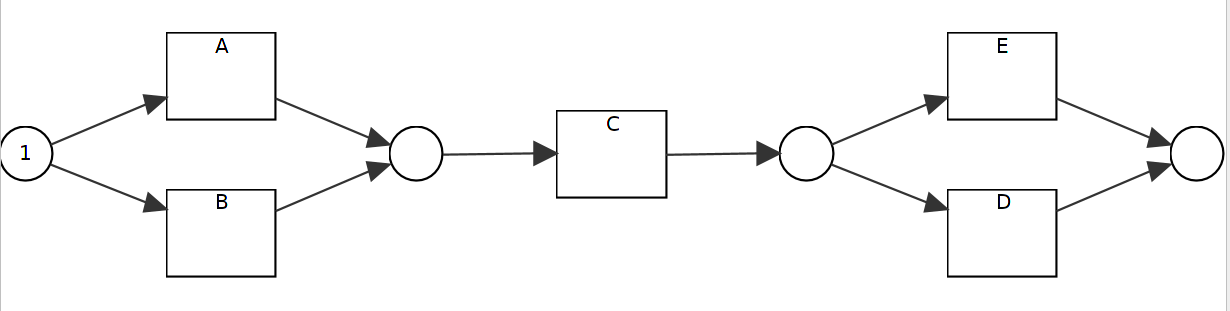
\includegraphics[width=\linewidth]{figures/preliminary/PN06_Seq_2_xor_notnested.png}
		\caption{A Simple Petri net}
		\label{fig:pn-seq-2}
	\end{subfigure}%
	\quad
	\begin{subfigure}[b]{0.45\textwidth}
		\centering
		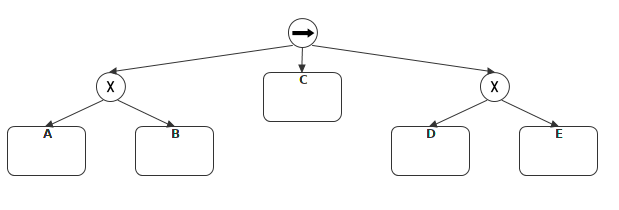
\includegraphics[width=\linewidth]{figures/preliminary/PT06_Seq_2_xor_notnested.png}
		\caption{A process tree corresponding to Fig \ref{fig:pn-seq-2}}
		\label{fig:pt-seq-2}
	\end{subfigure}%
\end{figure}
%% Here add the definition for soundness


\subsection{Process Tree}
Process tree is block-structured and sound by construction, while Petri nets, BPMN models possibly suffer from deadlocks, other anomalies\cite{van2016data}. Here we give the definition of process tree.
\begin{definition}[Process Tree]
Let $ A \subseteq \mathbb{A} $ be a finite set of activities with silent transition $\tau \in \mathbb{A}$, $\bigoplus \subseteq \{\rightarrow, \times, \land, \circlearrowright\}$ be the set of process tree operators. 
\begin{itemize}
\item $Q=a$ is a process tree with $a\in A$, and 
\item $Q= \oplus (Q_1 , Q_2 ,.. Q_n)$ is a process tree with $\oplus \in \bigoplus$, and $Q_i$ is a process tree, $i\in{1,2,..,n}, n\in \mathbb{N}$. 
\end{itemize}
\end{definition}

Process tree operators represents different block relation of each subtree. Their semantics are standardized from \cite{vanderAalst:2016:PMD:2948762, Buijs2012OnTR} and explained with use of Petri net in Figure \ref{fig:pn_pt_correspondings}\cite{Buijs2012OnTR}.
\begin{figure}[!h]
	\centering
	\begin{subfigure}[b]{0.45\textwidth}
		\centering
		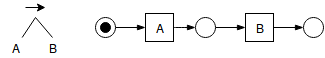
\includegraphics[width=\linewidth]{figures/preliminary/PT_PN_corresponding_01_seq_PN.png}
		\caption{Sequence}
		\label{fig:pt_pn_seq}
	\end{subfigure}%
	\quad
	\begin{subfigure}[b]{0.45\textwidth}
		\centering
		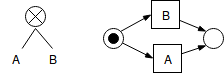
\includegraphics[width=\linewidth]{figures/preliminary/PT_PN_corresponding_02_xor_PN.png}
		\caption{Exclusive choice}
		\label{fig:pt_pn_xor}
	\end{subfigure}%
	\\ %this makes much difference
	\begin{subfigure}[b]{0.45\textwidth}
		\centering
		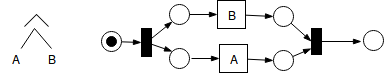
\includegraphics[width=\linewidth]{figures/preliminary/PT_PN_corresponding_03_and_PN.png}
		\caption{ Parallelism }
		\label{fig:pt_pn_and}
	\end{subfigure}%
	\quad
	\begin{subfigure}[b]{0.45\textwidth}
		\centering
		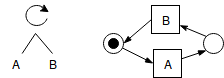
\includegraphics[width=\linewidth]{figures/preliminary/PT_PN_corresponding_04_loop_PN.png}
		\caption{Loop}
		\label{fig:pt_pn_loop}
	\end{subfigure}%
	\caption{Semantics of process tree operators w.r.t. Petri net}
	\label{fig:pn_pt_correspondings}
\end{figure}
\begin{definition}[Operator Semantics] 
	The semantics of operators $\bigoplus \subseteq \{\rightarrow, \times, \land, \circlearrowright \}$ are,
	\begin{itemize}
		\item if $Q= \rightarrow(Q_1 , Q_2 ,.. Q_n)$, the subtrees have sequential relation and are executed in order of $Q_1,Q_2,..Q_n$
		\item if $Q= \times(Q_1 , Q_2 ,.. Q_n)$,  the subtrees have exclusive choice relation and only one subtree of $Q_1,Q_2,..Q_n$   can be executed.
		\item if $Q= \land (Q_1 , Q_2 ,.. Q_n)$,  the subtrees have parallel relation and $Q_1,Q_2,..Q_n$ they can be executed in parallel.
		\item if $Q= \circlearrowright(Q_1 , Q_2 ,.. Q_n)$,  the subtrees have loop relation and $Q_1,Q_2,..Q_n \; with\; n\geq2$, $Q_1$ is the do-part and is executed at least once, $Q_2,..Q_n$ are redo part and have exclusive relation.
	\end{itemize}
\end{definition}
According to the corresponding semantic relations,  a process tree can be easily transformed into Petri net. In Figure \ref{fig:pt-seq-2}, it is the process model in process tree which describes the same process as in Figure \ref{fig:pn-seq-2}. 
%% here to describe the inductive miner 
\section{Inductive Miner}
To discover a process model from an event log, we choose one of the leading process discovery approaches -- Inductive Miner, because it guarantees the construction of a sound model, and is flexible and scalable to event log data. Its steps are listed bellow. 
\subsection{Construct a directly-follows graph}
A the start, the event log $L$ is scanned to extract the directly follows relation of events. The directly-follows relation is like the one in $\alpha$-algorithm \cite{van2004workflow, leemans2013discovering}, but the frequency information is stored for each relation. Later, those relations are combined together to build a directly-follows graph with frequency. According to \cite{van2016data, leemans2013discovering}, a directly-follows graph is defined bellow.
\begin{definition}[Directly-follows Graph]
 The directly-follows relation $a > b$ is satisfied iff there is a trace $\sigma\ where, \sigma(i)=a \ and \ \sigma(i+1)=b$.
 A directly-follows graph of an event log $L$ is $G(L) = (A, F, A_{start}, A_{end}) $ where $A$ is the set of activities in L, $F={(a,b) \in A \times A | a >_L b} $ is the directly-follows relation, $A_{start}, A_{end}$ are the set of start and end activities respectively.
\end{definition}
The frequency information of the directly-follows relation is called cardinality and defined below.
\begin{definition}[Cardinality in a directly-follows graph]
Given a directly-follows graph G(L) derived from an event log L, the cardinality of each directly-follows relation in G(L) is :  
	\begin{itemize}
		\item $Cardinality(E(A,B))$ is the frequency of traces with $\langle ...,A,B,... \rangle$. 
		\item Start node A cardinality $Cardinality(Start(A))$ is the frequency of traces with begin node A.
		\item End node B cardinality $Cardinality(End(A))$ is the frequency of traces with end node B.
	\end{itemize}	
\end{definition}
\subsection{Split Log Into Sublogs}
Based on the directly-follows graph, it finds the most prominent cut which is applied afterwards to split the event log into smaller sublogs. Cuts compose of \emph{exclusive-choice cut, sequence cut, parallel cut and redo-loop cut} which correspond to the process tree operators $ \{\rightarrow, \times, \land, \circlearrowright \}$. They are selected in the following order. A maximal exclusive-choice cut is firstly tried to split the directly-follows graph; if it is not available, then a maximal sequence cut, a  maximal parallel cut and a redo-loop cut are applied in sequence. Sublogs are created due to this available operator. Meanwhile, this operator is used to build the process tree. 

The same procedure is applied again on the sublogs until single activities. What's more, this process tree can be converted into Petri net for further analysis.